% !TeX spellcheck = en_US
\addsection{Expansion Content}{\skills/pathfinding.png}

\pagetarget{Expansion Content}
Numerous expansions have been released for Heroes III: The Board Game, introducing new gameplay elements.
Most expansion rules are integrated directly into the relevant sections of this rulebook where they belong.
Below you'll find an overview of all expansion content.

\textbf{The following contents are added by many of the expansions:}
\begin{multicols*}{2}
\subsection*{New Map Locations}
Each expansion adds new Map Locations to the game, which your Heroes can explore.
They are explained in \pagelink{All Map Locations}{All Map Locations}.

\subsection*{\pagetarget{Miniatures}{Unit Miniatures}}
If you want to play your Combats with Miniatures, place and move them over the Combat Board instead of the cards.
You can put Miniatures on top of the cards or keep the cards next to the Combat Board to form an initiative bar for better visualization of the order in which units activate.\par
\vspace*{1em}
If you play with Miniatures, there are a few rules to follow:
\begin{itemize}
  \item If any of the following occur during Combat with Neutral Units, discard the Neutral Unit card and draw another card in its place:
    \begin{itemize}
      \item if you draw the same Neutral Unit more than once,
      \item if you draw any unit you already have in your army,
      \item if you draw any unit from your Faction.
    \end{itemize}
  \item While you recruit Neutral Units, you cannot recruit any units from a Faction that is controlled by a player or any units that are already in any player's army.
  Discard that unit card and draw another.
\end{itemize}

\subsection*{Permanent cards}
Cards with a new type of effect which gives players permanent advantages, explained in \pagelink{Playerdecks}{Player Decks}.

\subsection*{Schools of Magic}
\pagelink{Schools of Magic}{Schools of Magic} gain more significance with the expansions, as there are now card effects which use them, e.g.~your Heroes can specialize in certain Schools to make their Spells more powerful.

\subsection*{Unique card effects with their own components}
Several new cards from various expansions come with their own Token components and bring complex effects to the game.
These are all explained in the separate section \pagelink{Detailed Card Effects}{Detailed Card Effects}.

\subsection*{More of the same}
In addition to new gameplay mechanics, expansions also expand the variety of existing components: new Factions, new Scenarios, new Spells, new Heroes, new Artifacts, and new Map Locations.

\begin{center}
    \includegraphics[width=0.75\linewidth]{\images/tower-lineup.png}
\end{center}
\vspace*{\fill}
\end{multicols*}
\pagebreak

\subheader{Factions Expansions}
\begin{multicols}{2}
\begin{expansion}[title=]{fortress}
  \subsection*{\color{fortress}Fortress Expansion}
  \setlength\intextsep{0pt}
  \setlength\columnsep{0.8em}
  \begin{wrapfigure}{l}{0.35\textwidth}
      \includegraphics[width=\linewidth]{\boxcovers/fortress-box.png}
  \end{wrapfigure}
  Contains the \textbf{Fortress Faction}: Poisonous swamp beasts under the command of Witches and Beastmasters.\par
  \medskip
  New gameplay mechanics: The new storytelling card type described below.
  \medskip
  \subsection*{\pagetarget{Events}{Events}}
  Event cards\index{Event cards} may be used in games with more than one player.
  Shuffle the Event Deck during setup.
  At the start of each Resource Round (except the first Round), draw and read the next Event card after receiving Resources.
  The first Event is drawn by the starting player.
  \textbf{Change the player who draws the Event in a clockwise order} every time a new Event is drawn.
  Resolve any effects in clockwise order starting with the player who drew the card.
  Any cards which were revealed as a part of resolving an Event should be shuffled back into their respective Decks afterwards.

  \medskip

  \begin{minipage}[h]{\linewidth}
  \vspace{0.1pt}
  \centering
  \begin{scriptsize}
    \begin{tikzpicture}
    \draw (0, 0) node[inner sep=0] {\makebox[\linewidth][c]{\includegraphics[width=\linewidth]{\cards/event.png}}};
    \draw (1, 1.8) node {\encircle{\phantom{.}1\phantom{.}}};
    \draw (-2, 0.4) node {\encircle{\phantom{.}2\phantom{.}}};
    \draw (2.5, -1.1) node {\encircle{\phantom{.}3\phantom{.}}};
    \end{tikzpicture}
  \end{scriptsize}
  \footnotesize
  \imagecaption{Event card}
  \begin{multicols}{2}
    \begin{itemize}
    \item[\textbf{1.}] Name
    \item[\textbf{2.}] Flavor text
    \item[\textbf{3.}] Effect
    \item[\textbf{\phantom{.}}] \phantom{.}
    \end{itemize}
  \end{multicols}
  \end{minipage}
\end{expansion}

\columnbreak
\begin{expansion}[title=]{rampart}
  \subsection*{\color{rampart}Rampart Expansion}
  \setlength\intextsep{0pt}
  \setlength\columnsep{0.8em}
  \begin{wrapfigure}{l}{0.35\textwidth}
    \includegraphics[width=\linewidth]{\boxcovers/rampart-box.png}
  \end{wrapfigure}
  Contains the \textbf{Rampart Faction}: Nature-oriented units under the lead of Druids and Rangers.\par
  \medskip
  New gameplay mechanics:\par
  \smallskip
  Various \pagelink{War Machines}{War Machines}, which support you with permanent effects in combat.
\end{expansion}

\vspace*{1em}
\begin{expansion}[title=]{inferno}
  \subsection*{\color{inferno}Inferno Expansion}
  \setlength\intextsep{0pt}
  \setlength\columnsep{0.8em}
  \begin{wrapfigure}{l}{0.35\textwidth}
    \includegraphics[width=\linewidth]{\boxcovers/inferno-box.png}
  \end{wrapfigure}
  Contains the \textbf{Inferno Faction}: Demonic and fire-associated units under the command of Heretics and Demoniacs.\par
  \medskip
  New gameplay mechanics:\par
  \smallskip
  A new unit Ability to \pagelink{Summoning}{Summon Demons} in combat; \pagelink{Empowered Statistic}{Empowered Statistic cards} to make your Hero's Statistic cards more powerful, and the \pagelink{Random Town}{Random Town} Map Location with unique combat rules.
\end{expansion}

\vspace*{1em}
\begin{expansion}[title=]{conflux}
  \subsection*{\color{conflux}Conflux Expansion}
  \setlength\intextsep{0pt}
  \setlength\columnsep{0.8em}
  \begin{wrapfigure}{l}{0.35\textwidth}
    \includegraphics[width=\linewidth]{\boxcovers/conflux-box.png}
  \end{wrapfigure}
  Contains the \textbf{Conflux Faction}: Magical Creatures of all elements under the command of Elementalists and Planeswalkers.\par
  \medskip
  New gameplay mechanics:\par
  \smallskip
  \pagelink{Elemental Map Tiles}{Elemental Map Tiles} aligned with Schools of Magic; magical \pagelink{Monolith Tokens}{Monoliths}, which allow your Heroes to traverse long distances on the Map; a new \pagelink{Elemental Damage}{type of damage} which ignores Defense; and a unique Spell effect to \pagelink{Detailed Card Effects}{Summon Elemental units}, which support you in combat.  % TODO: fix link
\end{expansion}
\vspace*{\fill}

\columnbreak
\begin{expansion}[title=]{stronghold}
  \subsection*{\color{stronghold}Stronghold Expansion}
  \setlength\intextsep{0pt}
  \setlength\columnsep{0.8em}
  \begin{wrapfigure}{l}{0.35\textwidth}
    \includegraphics[width=\linewidth]{\boxcovers/stronghold-box.png}
  \end{wrapfigure}
  Contains the \textbf{Stronghold Faction}: Wild and orkish units under command of Barbarians and Battle Mages.\par
  \medskip
  New gameplay mechanics:\par
  \smallskip
  \pagelink{Subterranean Map Tiles}{Subterranean Map Tiles}, which open a new world to explore, and mystical \pagelink{Spell Scroll Cards}{Spell Scrolls},
  which allow your Heroes to cast additional Spells even if they are not as familiar with magic.
\end{expansion}

\vspace*{1em}
\begin{expansion}[title=]{tower}
  \subsection*{\color{tower}Tower Expansion}
  \setlength\intextsep{0pt}
  \setlength\columnsep{0.8em}
  \begin{wrapfigure}{l}{0.35\textwidth}
    \includegraphics[width=\linewidth]{\boxcovers/tower-box.png}
  \end{wrapfigure}
  Contains the \textbf{Tower Faction}: Magic-oriented units under the lead of Wizards and Alchemists.\par
  \medskip
  This expansion doesn't introduce any new gameplay mechanics, but it expands many existing components, e.g.~it adds more \textbf{Heroes of other Factions}.
\end{expansion}
\vspace*{\fill}
\columnbreak

\begin{expansion}[title=]{cove}
  \subsection*{\color{cove}Cove Expansion}
  \setlength\intextsep{0pt}
  \setlength\columnsep{0.8em}
  \begin{wrapfigure}{l}{0.35\textwidth}
    \includegraphics[width=\linewidth]{\boxcovers/cove-box.png}
  \end{wrapfigure}
  Contains the \textbf{Cove Faction}: Pirate units and Sea monsters under the command of Captains and Navigators.\par
  \medskip
  New gameplay mechanics:\par
  \smallskip
  \pagelink{Sea Map Tiles}{Sea Map Tiles} with many new Sea Locations to discover; \pagelink{Whirlpool Tokens}{Whirlpools} to travel quickly between distant Sea Tiles… but \pagelink{Whirlpool}{at a cost}; and the Cannon, a new \pagelink{War Machines}{War Machine}.
\end{expansion}

\begin{center}
\hfill\transparent{0.2}\includegraphics[width=0.85\linewidth]{\art/earthquake.png}
\end{center}

\end{multicols}

\subheader{Gameplay and Game Mode Expansions}
\begin{multicols*}{2}
\begin{expansion}[title=]{navalbattles}
  \subsection*{\color{navalbattles}Naval Battles Expansion}
  \setlength\intextsep{0pt}
  \setlength\columnsep{0.8em}
  \begin{wrapfigure}{l}{0.35\textwidth}
    \includegraphics[width=\linewidth]{\boxcovers/navalbattles-box.png}
  \end{wrapfigure}
  This expansion offers three new gameplay mechanics:
  The \pagelink{Alternative Combat Boards}{Naval Battle Board} lets your Heroes fight Combat on ships, which is more challenging than on the normal Combat Board.
  The new \pagelink{Creature Banks Rules}{Creature Banks} Map Locations add challenging combats and \pagelink{Stack Tokens}{Stacked units}.
  The \pagelink{Empowered Ability Token}{empowered Ability cards} is a new reward.
\end{expansion}

\columnbreak
\begin{expansion}[title=]{battlefield}
  \subsection*{\color{battlefield}Battlefield Expansion}
  \setlength\intextsep{0pt}
  \setlength\columnsep{0.8em}
  \begin{wrapfigure}{l}{0.35\textwidth}
    \includegraphics[width=\linewidth]{\boxcovers/battlefield-box.png}
  \end{wrapfigure}
  The heart of this expansion is a large \pagelink{Battlefield Combat}{Battlefield Combat Board}. Two new \pagelink{Battlefield Modes}{game modes} are added around the use of this Battlefield Board, the rules for which must be consulted in the official rulebooks. Furthermore, the expansion offers an alternative \pagelink{Morale}{Morale gameplay system}, which you can use instead of the Morale Tokens.
\end{expansion}
\end{multicols*}

\pagebreak
\begin{expansion}[before=\vspace*{-11mm}]{navalbattles}
\pagetarget{Creature Banks Rules}{\subheader{Creature Banks}}
\begin{multicols*}{2}
  % \subsection*{\pagetarget{Creature Banks Rules}{Creature Banks}}
   Playing with Creature Banks is an \textbf{optional rule}.
   If you decide to play with Creature Banks, the following rules apply.

   \bigskip
   \subsection*{Setup}
   Separate the Creature Bank Tokens into two piles (for Near and Far Map Tiles) based on the numerals on their backs.
   Shuffle each pile and place them near the Map.
   Place the Creature Bank unit cards face up near the Neutral Unit Decks.
   There is no need to shuffle these cards.
   Shuffle all Stack Tokens and place them near the Creature Bank unit cards.

    \bigskip
    \begin{multicols*}{2}
      \begin{center}
        \includegraphics[width=1.0\linewidth]{\images/creature_bank_near.png}\\
        \vspace{-0.5em}\imagecaption{\footnotesize{}Creature Bank (Near)}\\
        \vspace*{\fill}
        \includegraphics[width=0.5\linewidth]{\images/stack_token.png}\\
        \imagecaption{\footnotesize{}Stack Token}\\
        \columnbreak
        \includegraphics[width=\linewidth]{\cards/creature_bank_unit.png}\\
        \imagecaption{\footnotesize{}Creature Bank unit card}
      \end{center}
    \end{multicols*}

  \subsection*{Placing Creature Bank Tokens}
  When you discover a Near or Far Map Tile, you may choose to draw a Creature Bank Token of the corresponding type, and place it on the Tile's Blocked Field.\par
  \begin{center}
  \vspace*{1em}
    \hspace*{-2em}\transparent{0.2}\includegraphics[width=0.9\linewidth]{\art/mermaid.png}
  \end{center}
  \columnbreak

  \subsection*{Visiting a Creature Bank\\Location}
  When you enter a Creature Bank Location, you must defeat the corresponding Creature Bank units defending it.
  If you win, resolve the Field's effect and mark it with a Black Cube.
  Because these Fields don't have any Difficulty Level, Quick Combat never happens, there is no Round limit, no need to spend MP to extend Combat, and you don't gain any \svg{experience}.
  The defending units and all effects of all Creature Bank Locations are listed in \pagelink{Creature Bank List}{All Map Locations}.

  \subsection*{Combat in a Creature Bank}
  When you start Combat at a Creature Bank, place up to 5 of your units in the player deployment zone.
  Depending on the Creature Bank you are visiting, take the corresponding units from the Creature Bank unit cards and place them randomly in the Neutral unit deployment zone.

    \bigskip
    \begin{center}
      \begin{tikzpicture}
        \draw (0, 0) node[inner sep=0] {\makebox[\linewidth][c]{\includegraphics[width=\linewidth]{\images/creature_bank_combat_board.png}}};
        \draw (-1.5, 0.6) node {\includegraphics[width=0.15\linewidth]{\images/P.png}};
        \draw (-1.5, -0.5) node {\includegraphics[width=0.15\linewidth]{\images/P.png}};
        \draw (0, 0.6) node {\includegraphics[width=0.15\linewidth]{\images/P.png}};
        \draw (0, -0.5) node {\includegraphics[width=0.15\linewidth]{\images/P.png}};
        \draw (1.5, 0.6) node {\includegraphics[width=0.15\linewidth]{\images/P.png}};
        \draw (1.5, -0.5) node {\includegraphics[width=0.15\linewidth]{\images/P.png}};
        \draw (2.9, 1.7) node {\includegraphics[width=0.15\linewidth]{\images/N.png}};
        \draw (2.9, -1.6) node {\includegraphics[width=0.15\linewidth]{\images/N.png}};
        \draw (-3.1, 1.7) node {\includegraphics[width=0.15\linewidth]{\images/N.png}};
        \draw (-3.1, -1.6) node {\includegraphics[width=0.15\linewidth]{\images/N.png}};
      \end{tikzpicture}
    \end{center}
    \imagecaption{\footnotesize{}P -- player deployment zone}\\
    \imagecaption{\footnotesize{}N -- Neutral Units deployment zone}\\
    \bigskip

  Based on the Scenario's Difficulty Level, take a number of \pagelink{Stack Tokens}{Stack Tokens} and place them randomly on up to four different Creature Bank unit cards:
  \begin{itemize}
    \item \textbf{Easy}: 1 token
    \item \textbf{Normal}: 2 tokens
    \item \textbf{Hard}: 3 tokens
    \item \textbf{Impossible}: 4 tokens
  \end{itemize}
  \end{multicols*}
\end{expansion}
\begin{expansion}[before=\vspace*{-11mm}]{navalbattles}
  \begin{multicols*}{2}
  After Combat, return all Creature Bank units back to the Creature Bank units cards pile.
  If you win, you claim the Creature Bank's reward, as well as an additional reward for the Stacked units you defeated.
  \subsection*{\pagetarget{Stack Tokens}{Stack Tokens}}
    \setlength\intextsep{0pt}
    \setlength\columnsep{1em}
    \begin{wrapfigure}{r}{0.2\linewidth}
      \includegraphics[width=\linewidth]{\images/stack_token.png}
    \end{wrapfigure}
  Each Stack Token modifies a unit's statistic in the following way: +1~\svg{attack}, +1~\svg{defense}, +1~\svg{health_points}, or +2~\svg{initiative}.
  Furthermore, each unit with a Stack Token is now a \textbf{Stacked unit}, which is similar to reinforced Faction units: when it takes damage equal to or greater than its \svg{health_points}, instead of removing the unit card from the Combat Board, discard the Stack Token from that unit and deal any leftover damage, deducting it from the new \svg{health_points}.
  Creature Bank units without a Stack Token are defeated normally.
  \columnbreak

  \subsection*{Gained Stacked Units}
  Some rewards allow you to gain a Stacked Creature Bank unit card.
  Track which of your units are Stacked by whatever means is comfortable, e.g.~by remembering it or by placing a Token or Cube on it.
  Whenever your Stacked unit goes to a Combat, draw a random Stack Token and place it on that unit.
  After Combat, note whether the unit is still Stacked (for future Combats), then return the Stack Token to the pile.
\end{multicols*}
\end{expansion}
\vfill
\hspace*{-1.2em}\includegraphics[width=1.05\textwidth]{\art/dread_knight.jpg}

\begin{expansion}{navalbattles}
\pagetarget{Empowered Ability Token}{\subheader{Empowered Ability Cards}}
\begin{multicols*}{2}
  This new type of card improves your Hero's Ability cards and is explained in \pagelink{Empowered Ability}{Deck-building}.

  \setlength\intextsep{0pt}
  \setlength\columnsep{1em}
  \begin{wrapfigure}{r}{0.2\linewidth}
    \includegraphics[width=\linewidth]{\images/crown-token.png}
  \end{wrapfigure}
  You can gain those cards by spending \textbf{Empowered Ability Tokens}.
  You can use one of these Tokens at the moment you gain a new Ability card, regardless of how you obtain it.
  If you use such a Token, discard it, remove the just-gained normal Ability card from the game, and gain the corresponding Empowered Ability card in its stead.
  There's only 1 copy of each Empowered Ability card, so if one player takes a particular Empowered Ability card, they prevent other players from obtaining it.
  If an Empowered Ability card isn't available, you can't spend the Empowered Ability Token and must keep it for later turns.

  You can gain Empowered Ability Tokens only in certain Scenarios (e.~g.~``Island of Fire'' from the Naval Battles Mission Book).\\

  \vspace*{5em}
  \begin{center}
    \transparent{0.2}\includegraphics[width=\linewidth]{\art/scholar.png}
  \end{center}

  \subsection*{Gaining Empowered Ability\\Example}
  \textit{Bob playing as Crag Hack reaches Level 2.
    He decides to perform the Search (2) action and draws two cards from the Ability Deck.
    The cards are Offense and Wisdom.
    He chooses Offense and places the other card on the discard pile.}

  \begin{center}
    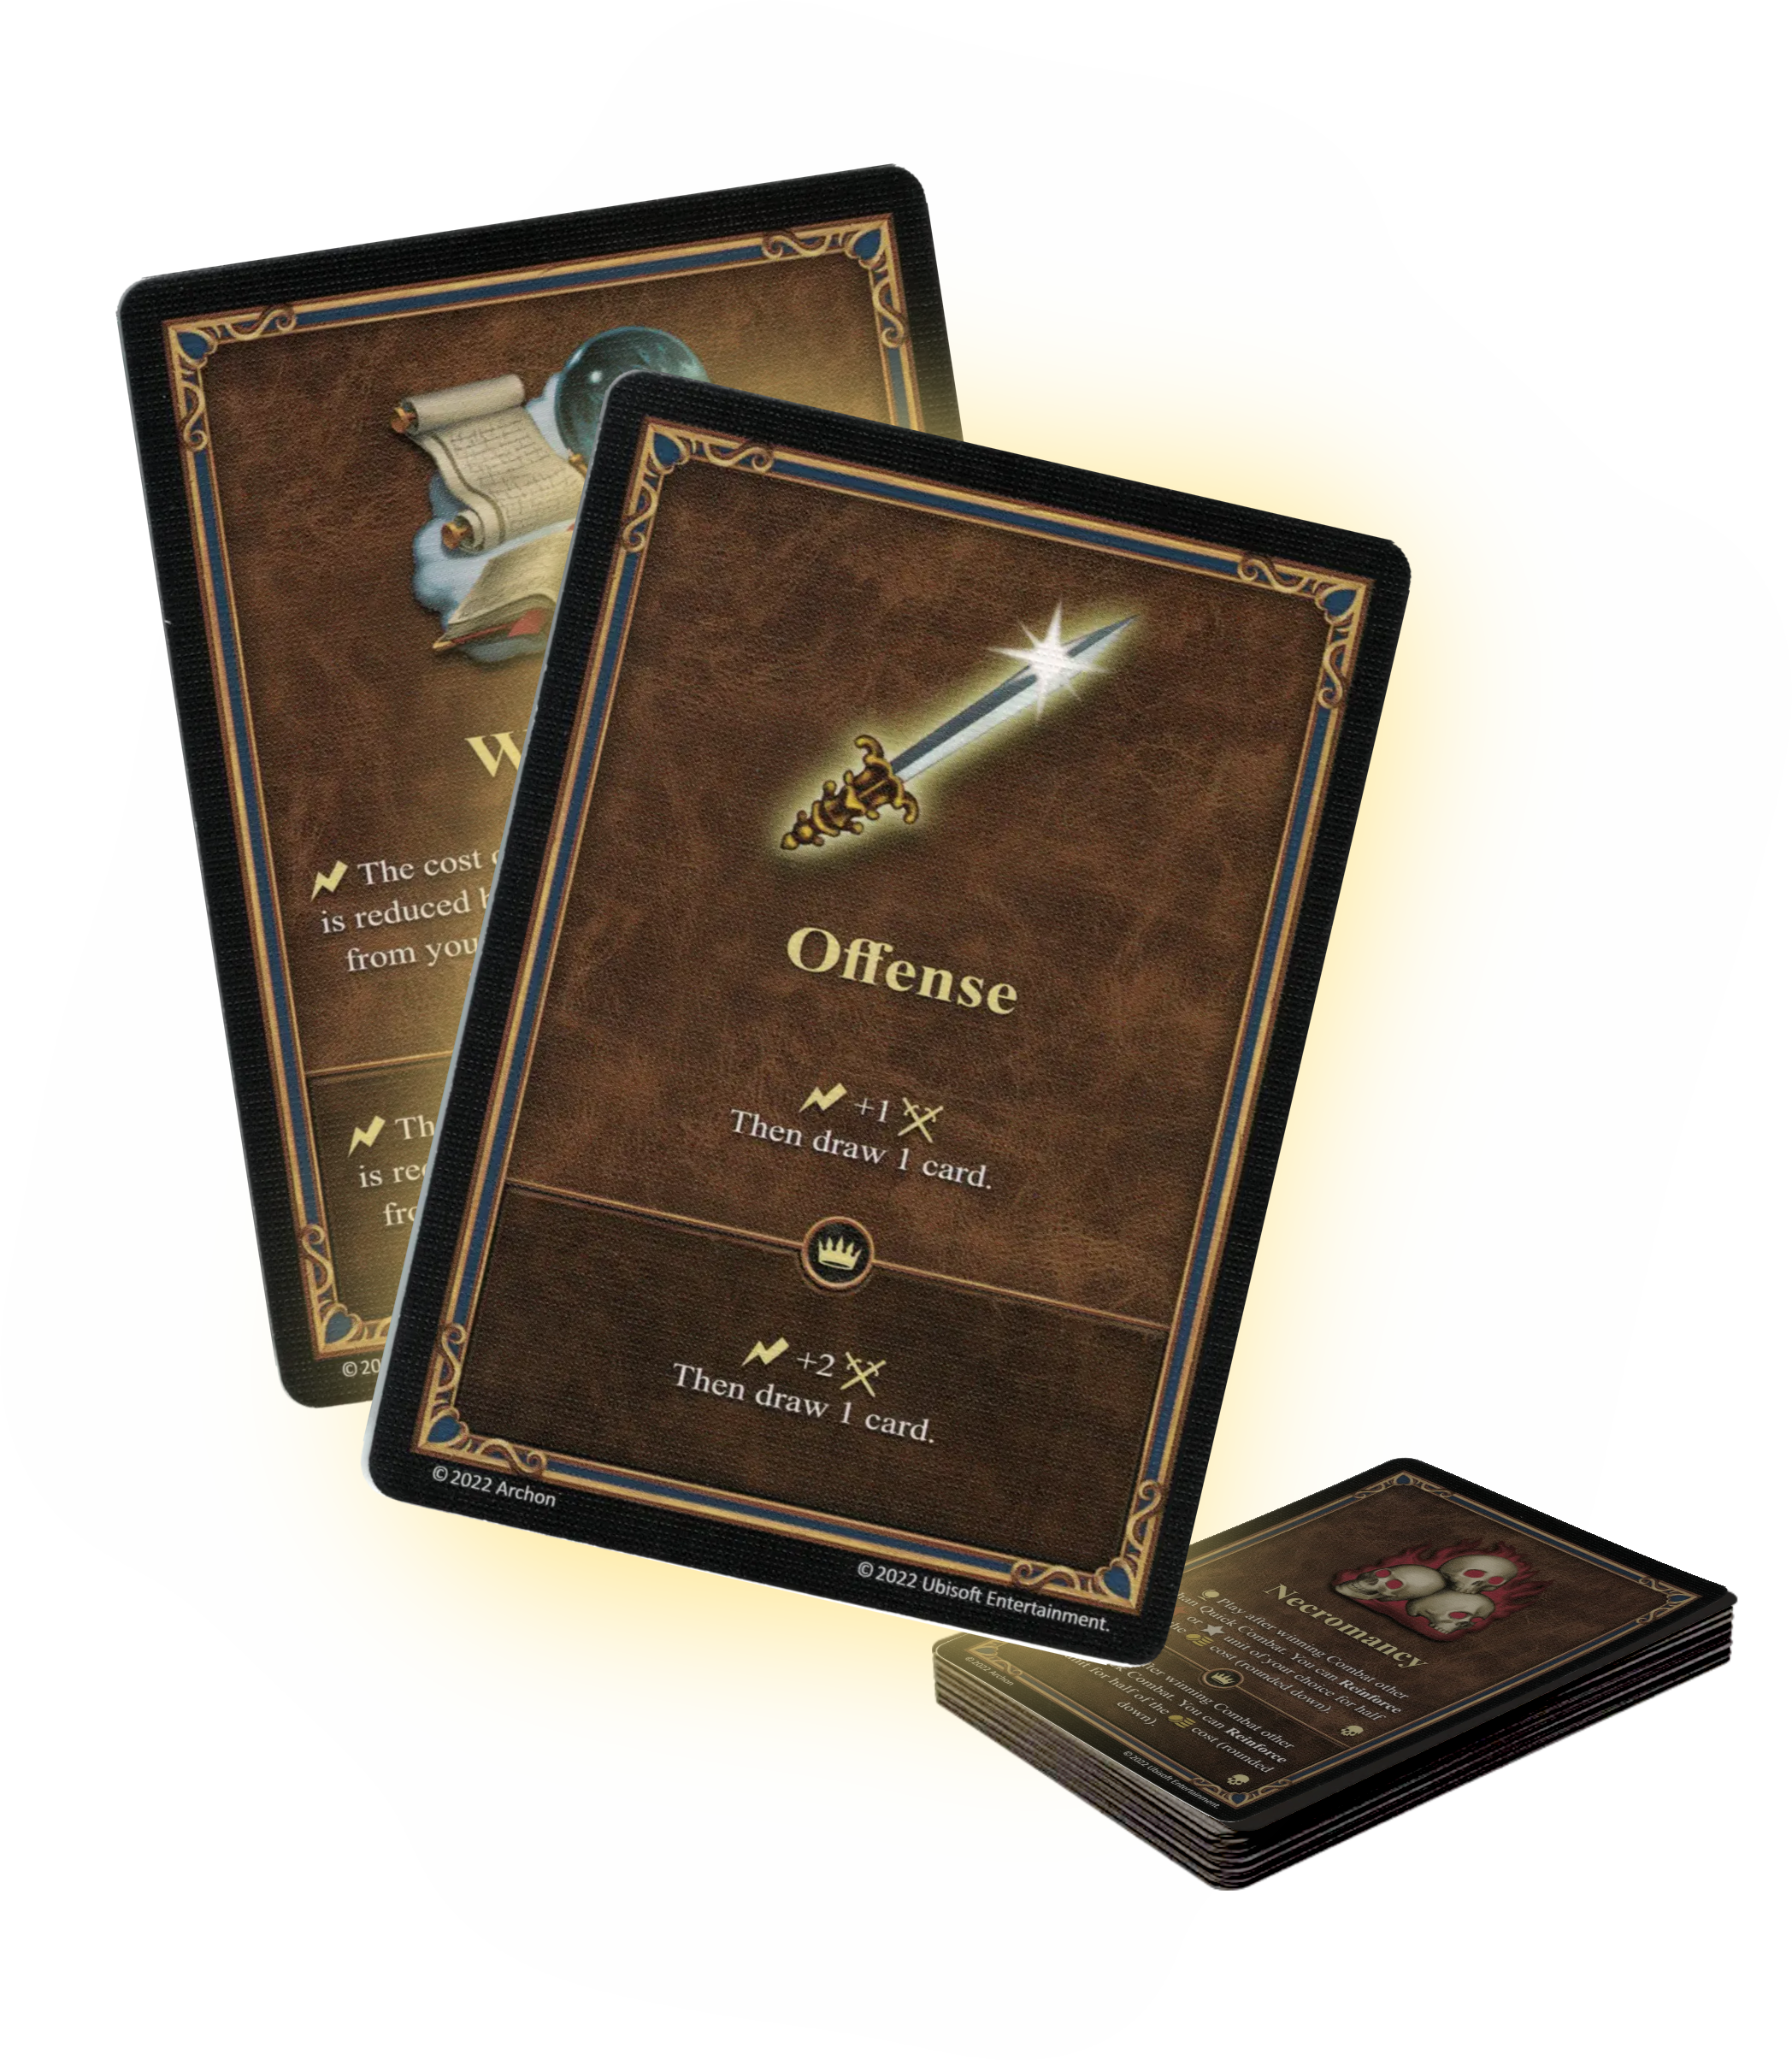
\includegraphics[width=0.8\linewidth]{\examples/offense_over_wisdom.png}
  \end{center}

  \textit{Bob happens to have an Empowered Ability Token.
    He may either use it, or save the token for later.
    He decides to use it, so he removes the ``Offense'' Ability card and take the Empowered ``Offense'' Ability card instead.}

  \begin{center}
    \begin{tikzpicture}
      \draw (-2, 0) node {\includegraphics[width=0.3\linewidth]{\cards/ability-offense.png}};
      \draw (-3, -0.5) node[circular drop shadow={shadow scale=0.8, shadow xshift=0.3ex, shadow yshift=-0.3ex, opacity=0.7,
        fill=black, path fading={circle with fuzzy edge 15 percent},
        every shadow}]{\includegraphics[width=0.15\linewidth]{\images/crown-token.png}};
      \draw (-3.7, -1) node[rotate=87, xscale=-1] {\includegraphics[width=0.2\linewidth]{\_assets/gimp-files/arrow-curved-red.png}};
      \draw (2, 0) node {\includegraphics[width=0.3\linewidth]{\cards/ability-offense-empowered.png}};
      \draw (3, 1) node[circular drop shadow={shadow scale=0.8, shadow xshift=0.3ex, shadow yshift=-0.3ex, opacity=0.5,
        fill=black, path fading={circle with fuzzy edge 15 percent},
        every shadow}] {\svg[25]{green_tick}};
    \end{tikzpicture}
  \end{center}
  \vspace*{\fill}
\end{multicols*}
\end{expansion}

\pagebreak
\begin{expansion}[before=\vspace*{-11mm}]{battlefield}
  \pagetarget{Battlefield Combat}{\subheader{Combat on the Battlefield Board}}
  \begin{multicols*}{2}
  \textbf{Note:} The rules for \pagelink{Battlefield Modes}{Skirmish and Adventure} are different from this, please check the official rulebook.

  \medskip
  It is recommended to use the Battlefield Combat Board only for \textbf{Player vs.~Player Combats}, even though it is also possible to use it in Neutral Combats.
  Using the Battlefield Board requires using \pagelink{Miniatures}{Miniatures} instead of unit cards.

  \subsection*{Battlefield Board in Neutral\\Combats}
  If you decide to use the Battlefield Board in Combats with Neutral Units, ignore the Round Limit:
  At the end of each Combat Round you may freely decide to Retreat or to gain an additional Combat Round with no need to spend a MP \svg{movement}.
  Be aware, however, that this may significantly extend the playtime.

  \subsection*{\pagetarget{BF Obstacles}{Obstacle Tokens}}
  On the Battlefield Board you place Obstacle Tokens, which are divided into three types:
  Effect, Obstacle and Wall/Gate.
  Unless otherwise stated these Tokens count and work as \pagelink{Combatterminology}{Combat Obstacles}.
  To place Effect Obstacles on the Battlefield Board you'll need the card which creates the effect, such as the Fire Wall Spell: use the Tokens and put the Card beside the Battlefield as a reminder.
  Effect Obstacles may be entered by Units, if the Card text allows it.
  \begin{figure}[H]
    \centering
    \begin{subfigure}[b]{0.3\linewidth}
      \centering
      \includegraphics[width=0.7\linewidth]{\images/bf-obstacle-1.png}
      \caption{\imagecaption{Effect}}
    \end{subfigure}
    \begin{subfigure}[b]{0.3\linewidth}
      \centering
      \includegraphics[width=0.9\linewidth]{\images/bf-obstacle-2.png}
      \caption{\imagecaption{Obstacle}}
    \end{subfigure}
    \begin{subfigure}[b]{0.3\linewidth}
      \centering
      \includegraphics[width=0.9\linewidth]{\images/bf-obstacle-3.png}
      \caption{\imagecaption{Wall/Gate}}
    \end{subfigure}
  \end{figure}
  \note{3}{
    All unit Miniatures also count as Obstacles.
  }
  \columnbreak

  \subsection*{Rules Changes in Combat Setup}
  \begin{itemize}
    \item \textbf{Place obstacles} – Starting with the attacking player, both players take turns choosing and placing one Obstacle Token on the Battlefield Board until \textbf{all Obstacle Tokens (no Effects yet) are placed}.
    No Obstacle can be adjacent to another Obstacle or to any player's deployment zone.

    \begin{tikzpicture}
      \draw (0, 0) node {\includegraphics[width=0.9\linewidth]{\examples/bf-deploy.png}};
      \draw (2.5, 0) node[rotate=90] {\textbf{\fontfamily{ptm}\selectfont\textcolor{white}{DEPLOYMENT ZONE}}};
    \end{tikzpicture}
    {\footnotesize\imagecaption{Obstacles and models placed correctly are marked with the green border, and incorrectly -- with the red one.}}
    \item \textbf{Place units} – Starting from the attacking player, the players choose a deployment zone and take turns placing their units \textbf{one by one}.
    When the last unit is placed, the Combat begins.
    Only in Player vs. Player Combats can the players decide to allow placing \textbf{up to 7 units} (instead of 5).
  \end{itemize}
  \end{multicols*}
\end{expansion}

\newpage
\begin{expansion}[before=\vspace*{-11mm}]{battlefield}
  \begin{multicols*}{2}
  \begin{itemize}
    \item \textbf{Siege with Walls and Gate} – During a Siege against a Town with a Citadel, only Walls and Gate Obstacles are placed.
      Place no other Obstacles.

    \begin{tikzpicture}
      \draw (0, 0) node {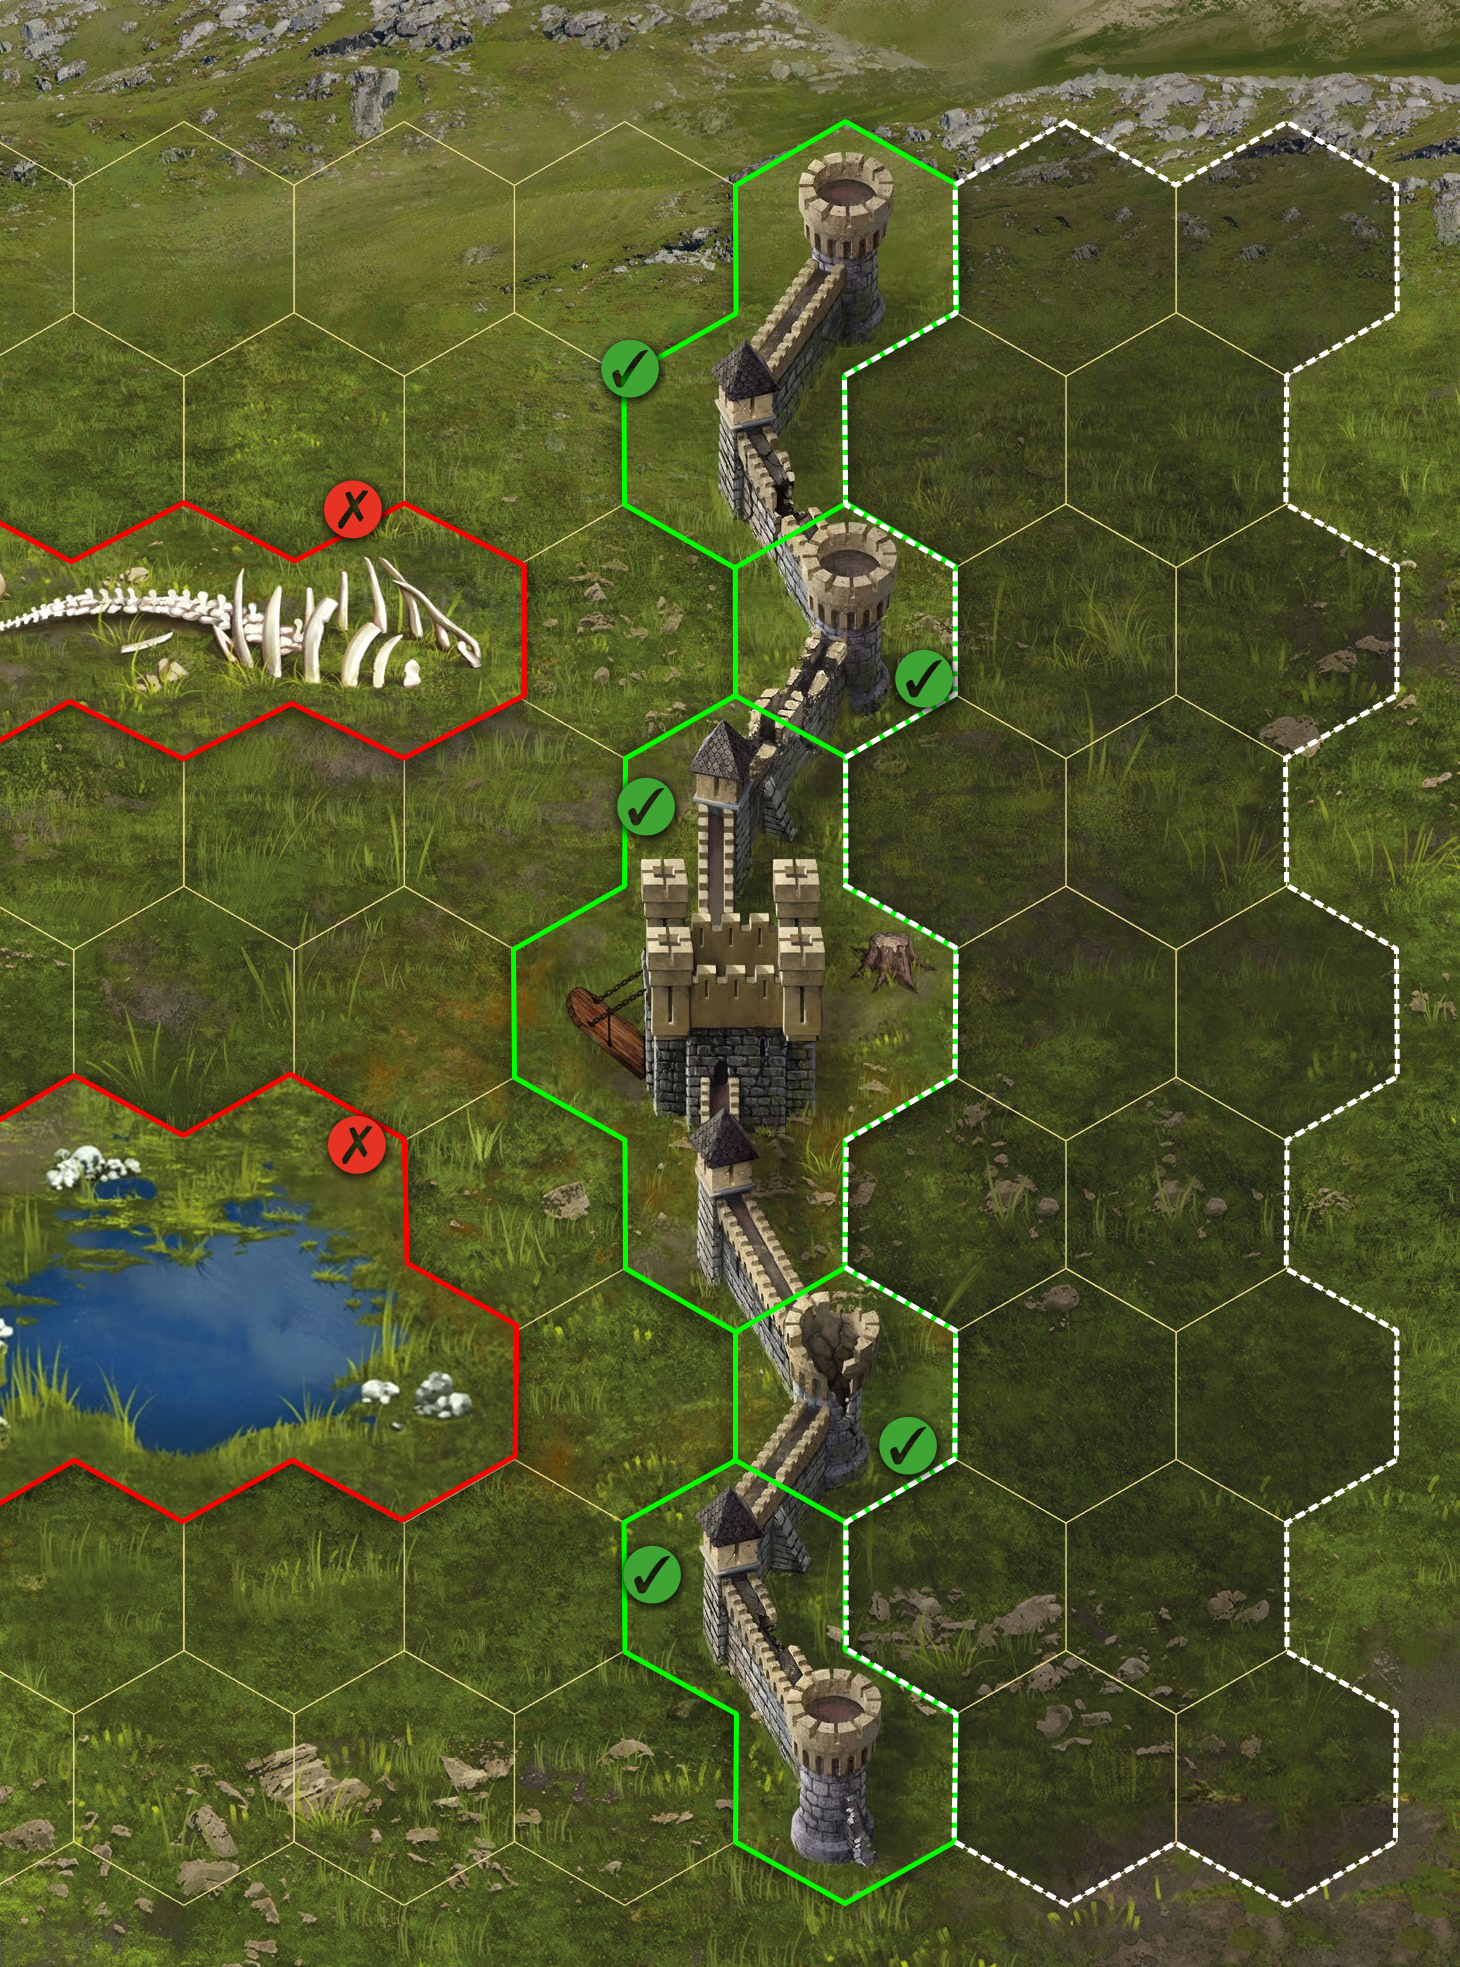
\includegraphics[width=1.05\linewidth]{\examples/bf-deploy-wall.png}};
      \draw (2, 0) node[rotate=90] {\textbf{\fontfamily{ptm}\selectfont\textcolor{white}{DEPLOYMENT ZONE}}};
    \end{tikzpicture}
    {\footnotesize\imagecaption{The red border marks incorrectly placed Obstacles.}}
  \end{itemize}
  \subsection*{Rules Changes during Combat}
  \begin{itemize}
    \item \textbf{Unit Movement} – Each unit's Movement is equal to its Initiative value: a unit of Initiative 8 can move up to 8 hexes.
    \item \textbf{Ranged Movement}  – Ranged \svg{unit_ranged} units can either move or attack, not both.
    \item \textbf{Combat Penalty} – Ranged \svg{unit_ranged} units suffer a Combat Penalty when attacking an adjacent unit or a unit that is \textbf{8 or more} hexes away from them.
    \begin{center}
      \vspace*{1em}
      \transparent{0.2}\includegraphics[width=0.7\linewidth]{\art/land_mine.png}
    \end{center}
    \columnbreak

    \begin{minipage}{\linewidth}
      \setlength\intextsep{0pt}
      \setlength\columnsep{1em}
      \begin{wrapfigure}{r}{0.3\linewidth}
        \includegraphics[width=\linewidth]{\images/initiative-bf.png}
      \end{wrapfigure}
      \item \textbf{\pagetarget{Initiative Token}{Initiative Token}} – At the start of Combat, the attacking player gains the Initiative Token.
      Use it only to break any Initiative ties of opposing units:
      The player with the Token activates first \textbf{one of their units of the same Initiative value}.
      Then, the players alternate in activating all of their units of that same Initiative value one by one.
      Once all units with that Initiative value are activated, pass the Initiative Token to the other player, who keeps it until initiative ties must be resolved again in the same way.
    \end{minipage}

    \item \textbf{Gate Token} – During a Siege, defending units may enter the Gate Token \textbf{only at the two middle hexes} where the Gate is printed.
    Attacking the Gate Token is still possible on all four hexes.

    \vspace*{1em}
    \includegraphics[width=\linewidth]{\examples/bf-gate-token.png}
    \footnotesize\textit{Example: Halberdier and Crusader (defenders) may enter the Gate Token only along the green arrows, but Minotaur and Harpies are still able to attack the Gate Token from any side.}
  \end{itemize}
    \vspace*{\fill}
  \end{multicols*}
\end{expansion}

\newpage
\begin{multicols}{2}

\subheader{Stretch Goal Content}

Four boxes of stretchgoal content have been released for the boardgame; they are shown at the bottom of this page.\par
These expansions primarily contain aesthetic components (like Miniatures of Neutral Units or Map Locations), but they also extend the variety of existing components (like additional Artifact or Spell cards or new Hero Boards for all Factions).\par
\smallskip

The only new gameplay element from a Stretchgoal box is explained below:\par
\vspace*{1em}
 \begin{expansion}{stretchgoals2}
   \subsection*{\pagetarget{Pandora Card}{Pandora's Box cards}}
   During setup, shuffle the Pandora's Box cards.
   When you Visit a \pagelink{Pandora Box}{Pandora's Box}, you may optionally draw a Pandora's Box card and resolve it instead of the location's regular effect.
   You still have to mark the Field with a Black Cube.

   \medskip
   \begin{center}
     \includegraphics[width=0.6\linewidth]{\cards/pandora.png}
   \end{center}
 \end{expansion}
 \vspace*{\fill}
 \columnbreak
\subheader{Fan-Made Content}
Take a look at the \textbf{fan-made expansions and content} from the \textbf{HoMM3 BG Community}.
  \begin{itemize}
    \begin{minipage}{5cm}
      \item The \textbf{Fan-Made Mission Book} contains many well-playtested Scenarios with unique rules for even more spice in your games:
      \mbox{\footnotesize \href{https://github.com/qwrtln/Homm3BG-mission-book}{github.com/qwrtln/Homm3BG-mission-book}}
    \end{minipage}
    \hfill
    \begin{minipage}{2cm}
        \begin{center}
            \includegraphics[width=\linewidth]{\qr/mission-book.png}
            \scriptsize \phantom{Link to \textbf{Github}}
        \end{center}
    \end{minipage}\par
    \smallskip
    \begin{minipage}{5cm}
      \item The \textbf{Fan-Made Factory Expansion} introduces the missing Faction.
      Print it yourself and learn a new Faction to master:
      {\footnotesize \href{https://github.com/piotrbruzda/Homm3BG-FactoryRulebook}{github.com/piotrbruzda/Homm3BG-FactoryRulebook}}
    \end{minipage}
    \hfill
    \begin{minipage}{2cm}
        \begin{center}
            \vspace*{-1em}
            \includegraphics[width=\linewidth]{\qr/factory.png}
            \scriptsize \phantom{Link to \textbf{Github}}
        \end{center}
    \end{minipage}\par
    \smallskip
  \end{itemize}
  \begin{center}
    \vspace*{-0.5em}
    \hfill\includegraphics[width=0.85\linewidth]{\images/mission-book-with-factory.png}
  \end{center}
  \begin{itemize}
    \begin{minipage}{5cm}
        \item Bring your creative ideas to life by building your own Scenarios with the help of the \textbf{Scenario Map Editor}:
        {\footnotesize \href{https://zedero.github.io/homm3boardgame/}{zedero.github.io/homm3boardgame}}
    \end{minipage}
    \hfill
    \begin{minipage}{2cm}
        \begin{center}
            \includegraphics[width=\linewidth]{\qr/map-editor.png}
            \scriptsize \phantom{Link to the \textbf{App}}
        \end{center}
    \end{minipage}\par
    \smallskip
    \begin{minipage}{5cm}
    \item Generate your own custom Heroes and their unique Specialties with the \textbf{Hero Creator} and let them make history:
      \mbox{\footnotesize \href{https://k-adam.github.io/Homm3_hero_creator}{k-adam.github.io/Homm3\textunderscore{}hero\textunderscore{}creator}}
    \end{minipage}
    \hfill
    \begin{minipage}{2cm}
        \begin{center}
            \includegraphics[width=\linewidth]{\qr/hero-creator.png}
            \scriptsize \phantom{Link to the \textbf{App}}
        \end{center}
    \end{minipage}\par
  \end{itemize}
\end{multicols}
\begin{multicols}{4}
    \begin{center}
        \includegraphics[width=0.8\linewidth]{\boxcovers/stretchgoals-factionunits.png}\newline
        \footnotesize Core Game Faction Miniatures\par
        \columnbreak
        \includegraphics[width=0.8\linewidth]{\boxcovers/stretchgoals-neutral.png}\newline
        \footnotesize \nth{1} Campaign Miniatures\par
        \columnbreak
        \includegraphics[width=0.8\linewidth]{\boxcovers/stretchgoals-chest.png}\newline
        \footnotesize \nth{2} Campaign \mbox{Gameplay Components}\par
        \columnbreak
        \includegraphics[width=0.8\linewidth]{\boxcovers/stretchgoals-crystal.png}\newline
        \footnotesize \nth{2} Campaign Miniatures\par
    \end{center}
\end{multicols}
